\documentclass[preview]{standalone}
\usepackage{tikz}
\usepackage{xcolor}

\definecolor{tealish}{HTML}{64d8cb}
\definecolor{fillteal}{HTML}{b2f0ea} % a lighter fill version of tealish

\begin{document}

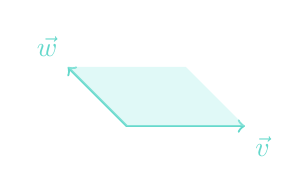
\begin{tikzpicture}[scale=1.5, line cap=round]
  % Vectors
  \draw[->, thick, tealish] (0,0) -- (1,0) node[below right] {$\vec{v}$};
  \draw[->, thick, tealish] (0,0) -- (-0.5,0.5) node[above left] {$\vec{w}$};
  
  % Shade parallelogram
  \fill[fillteal, opacity=0.4] 
  (0,0) 
  -- (1,0) 
  -- (0.5,0.5) 
  -- (-0.5,0.5) 
  -- cycle;
\end{tikzpicture}

\end{document}
